\begin{surferIntroPage}{Tutorial}{tutorial_koord1}{First steps with SURFER}
This program is called SURFER. If you read this word you probably think of water, sun and waves. In this case the name comes from the word {\it surface}.
\\
With SURFER one can display surfaces, more precisely algebraic surfaces. What this means and what algebraic surfaces are, is explained in this tutorial. Choose one of the surfaces on the right side to browse through the chapters of this tutorial.\\
SURFER is part of the travelling exhibition IMAGINARY which started in the German Year of Mathematics 2008. The exhibition is a project by the internationally known Mathematisches Forschungsinstitut Oberwolfach situated in the German black forest. Every week workshops to recent topics in mathematical research are held at the institute. These workshops are important to foster exchange between scientists all around the world. \\
\vspace{0.2cm} \hspace{3.5cm}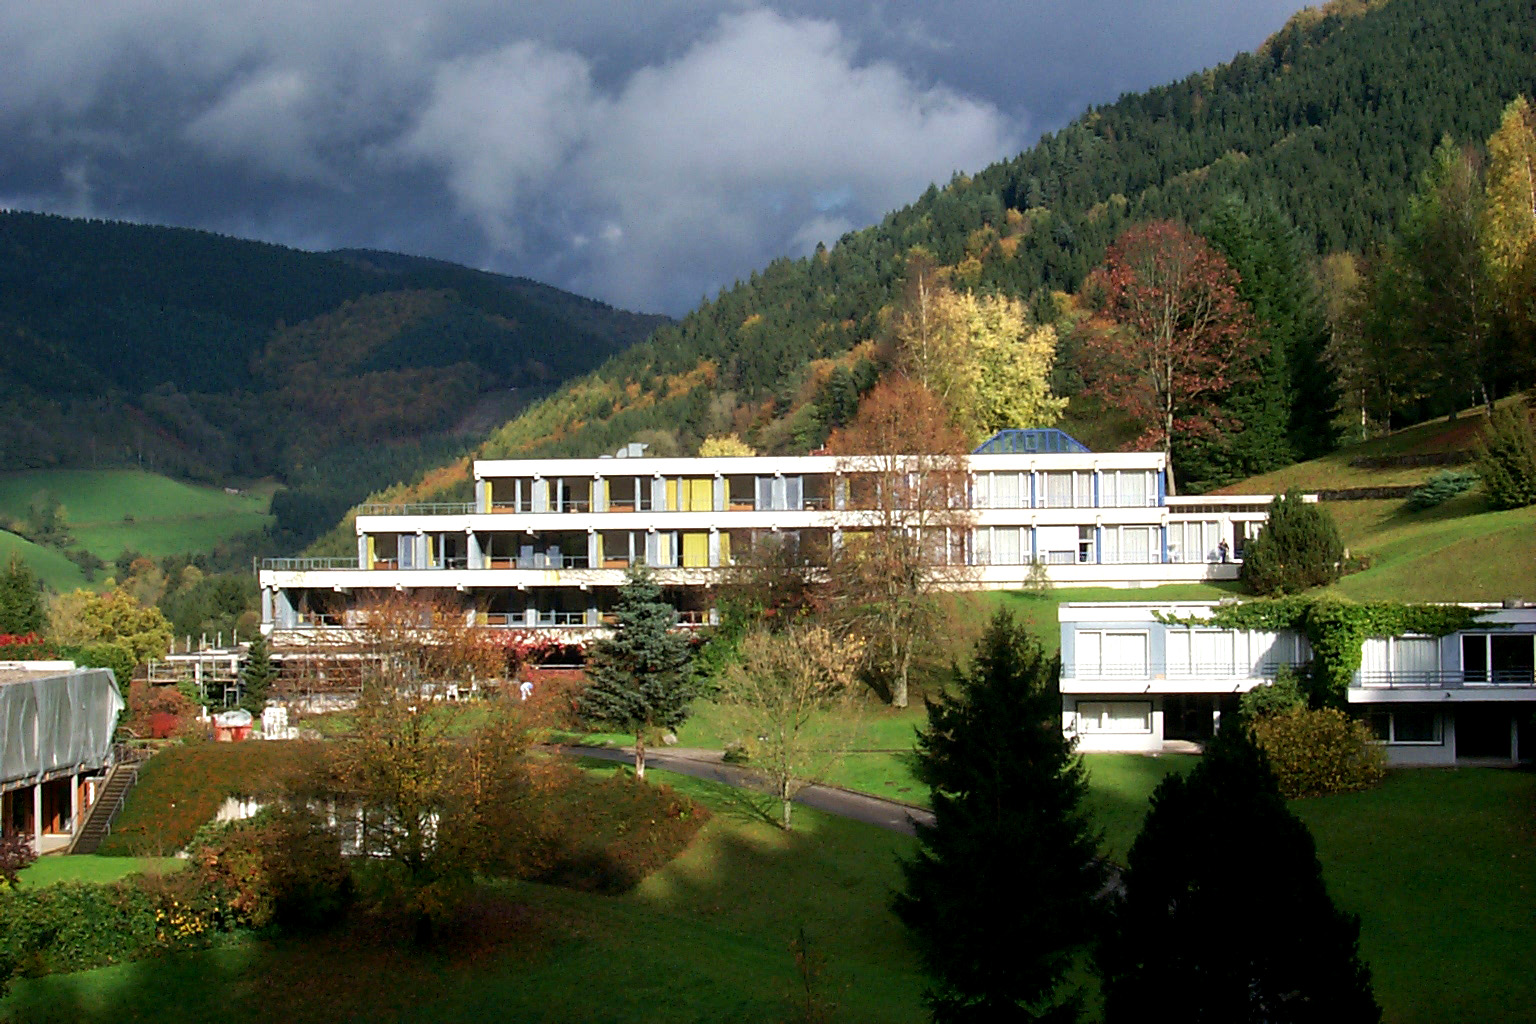
\includegraphics[width=3cm]{./../../common/images/photo_mfo.jpg}\\
The SURFER programme can be downloaded for free at our homepage: \\
\begin{centering}
www.imaginary-exhibition.com\\
\end{centering}
 \vspace{0.2cm}
On your right you can choose one of the mathematical tutorials starting with the Zitrus surface. On your left you can jump to other galleries, for example the gallery of fantasy surfaces.
\end{surferIntroPage}
